\documentclass[floatsintext,man]{apa6}

\usepackage{amssymb,amsmath}
\usepackage{ifxetex,ifluatex}
\usepackage{fixltx2e} % provides \textsubscript
\ifnum 0\ifxetex 1\fi\ifluatex 1\fi=0 % if pdftex
  \usepackage[T1]{fontenc}
  \usepackage[utf8]{inputenc}
\else % if luatex or xelatex
  \ifxetex
    \usepackage{mathspec}
    \usepackage{xltxtra,xunicode}
  \else
    \usepackage{fontspec}
  \fi
  \defaultfontfeatures{Mapping=tex-text,Scale=MatchLowercase}
  \newcommand{\euro}{€}
\fi
% use upquote if available, for straight quotes in verbatim environments
\IfFileExists{upquote.sty}{\usepackage{upquote}}{}
% use microtype if available
\IfFileExists{microtype.sty}{\usepackage{microtype}}{}

% Table formatting
\usepackage{longtable, booktabs}
\usepackage{lscape}
% \usepackage[counterclockwise]{rotating}   % Landscape page setup for large tables
\usepackage{multirow}		% Table styling
\usepackage{tabularx}		% Control Column width
\usepackage[flushleft]{threeparttable}	% Allows for three part tables with a specified notes section
\usepackage{threeparttablex}            % Lets threeparttable work with longtable

% Create new environments so endfloat can handle them
% \newenvironment{ltable}
%   {\begin{landscape}\begin{center}\begin{threeparttable}}
%   {\end{threeparttable}\end{center}\end{landscape}}

\newenvironment{lltable}
  {\begin{landscape}\begin{center}\begin{ThreePartTable}}
  {\end{ThreePartTable}\end{center}\end{landscape}}




% The following enables adjusting longtable caption width to table width
% Solution found at http://golatex.de/longtable-mit-caption-so-breit-wie-die-tabelle-t15767.html
\makeatletter
\newcommand\LastLTentrywidth{1em}
\newlength\longtablewidth
\setlength{\longtablewidth}{1in}
\newcommand\getlongtablewidth{%
 \begingroup
  \ifcsname LT@\roman{LT@tables}\endcsname
  \global\longtablewidth=0pt
  \renewcommand\LT@entry[2]{\global\advance\longtablewidth by ##2\relax\gdef\LastLTentrywidth{##2}}%
  \@nameuse{LT@\roman{LT@tables}}%
  \fi
\endgroup}


  \usepackage{graphicx}
  \makeatletter
  \def\maxwidth{\ifdim\Gin@nat@width>\linewidth\linewidth\else\Gin@nat@width\fi}
  \def\maxheight{\ifdim\Gin@nat@height>\textheight\textheight\else\Gin@nat@height\fi}
  \makeatother
  % Scale images if necessary, so that they will not overflow the page
  % margins by default, and it is still possible to overwrite the defaults
  % using explicit options in \includegraphics[width, height, ...]{}
  \setkeys{Gin}{width=\maxwidth,height=\maxheight,keepaspectratio}
\ifxetex
  \usepackage[setpagesize=false, % page size defined by xetex
              unicode=false, % unicode breaks when used with xetex
              xetex]{hyperref}
\else
  \usepackage[unicode=true]{hyperref}
\fi
\hypersetup{breaklinks=true,
            pdfauthor={},
            pdftitle={Instance theory predicts information theory: Episodic uncertainty as a determinant of keystroke dynamics},
            colorlinks=true,
            citecolor=blue,
            urlcolor=blue,
            linkcolor=black,
            pdfborder={0 0 0}}
\urlstyle{same}  % don't use monospace font for urls

\setlength{\parindent}{0pt}
%\setlength{\parskip}{0pt plus 0pt minus 0pt}

\setlength{\emergencystretch}{3em}  % prevent overfull lines


% Manuscript styling
\captionsetup{font=singlespacing,justification=justified}
\usepackage{csquotes}
\usepackage{upgreek}



\usepackage{tikz} % Variable definition to generate author note

% fix for \tightlist problem in pandoc 1.14
\providecommand{\tightlist}{%
  \setlength{\itemsep}{0pt}\setlength{\parskip}{0pt}}

% Essential manuscript parts
  \title{Instance theory predicts information theory: Episodic uncertainty as a
determinant of keystroke dynamics}

  \shorttitle{Episodic Uncertainty and Performance}


  \author{Matthew J. C. Crump\textsuperscript{1}, Walter Lai\textsuperscript{1}, \& Nicholaus Brosowsky\textsuperscript{1}}

  % \def\affdep{{"", "", ""}}%
  % \def\affcity{{"", "", ""}}%

  \affiliation{
    \vspace{0.5cm}
          \textsuperscript{1} Brooklyn College of the City University of New York  }

  \authornote{
    In this draft, listed authorship order simply indicates who is
    participating in the project
    
    Correspondence concerning this article should be addressed to Matthew J.
    C. Crump, Brooklyn College of CUNY, 2900 Bedford Avenue, Brooklyn, NY,
    11210. E-mail:
    \href{mailto:mcrump@brooklyn.cuny.edu}{\nolinkurl{mcrump@brooklyn.cuny.edu}}
  }


  \abstract{Enter abstract here. Each new line herein must be indented, like this
line.}
  \keywords{Instance Theory, Information Theory, Entropy, Uncertainty, Typing,
Performance \\

    \indent Word count: X
  }





\usepackage{amsthm}
\newtheorem{theorem}{Theorem}
\newtheorem{lemma}{Lemma}
\theoremstyle{definition}
\newtheorem{definition}{Definition}
\newtheorem{corollary}{Corollary}
\newtheorem{proposition}{Proposition}
\theoremstyle{definition}
\newtheorem{example}{Example}
\theoremstyle{definition}
\newtheorem{exercise}{Exercise}
\theoremstyle{remark}
\newtheorem*{remark}{Remark}
\newtheorem*{solution}{Solution}
\begin{document}

\maketitle

\setcounter{secnumdepth}{0}



Theories of cognitive processes run along a continuum. On one extreme,
cognitive phenomena are explained in terms specialized and dedicated
modules (Fodor, 1983) that give rise to cognition by the principles of
their internal processing architecture. On the other extreme, cognitive
phenomena are explained in terms of general learning and memory
processes (Jacoby \& Brooks, 1984; Kolers \& Roediger, 1984; Rumelhart
\& McClelland, 1986) that give rise to cognition through their
experience with a structured environment (Clark, 2008). Valid theories
produce explanations of phenomena by deduction from their processing
assumptions, and then compete with other valid theories on the basis of
parsimony. When a phenomena is explained by a general process,
specialized accounts become sufficient, but not necessary; and, vice
versa. We continue in this tradtion by proposing and validating a
general process account of keystroke dynamics in skilled typing
performance. We show that keystroke dynamics can emerge from a general
memory process sensitive to structure (uncertainty) in the natural
language environment.

We identified the following pre-requisites as necessary for our
approach. We follow the assumption that specialized or general processes
of cognition are constrained to operate upon the structure of their
environmental inputs. So, we require a tool for describing the structure
of environmental inputs. We assume that performance is driven by
learning processes sensitive to the structure in the environment. So, we
require a model that articulates how learning about the structure of an
environment produces performance. Finally, we require a task where the
relation between performance and a structured environment can be
measured. We use information theory (Shannon \& Weaver, 1998) to measure
the structure of the letters that typists' type, instance theory (Logan,
1988) to model how typists' performance is shaped by the typing
environment, and the task of continuous typing (Logan \& Crump, 2011) to
measure keystroke dynamics as a function of the structure in the typing
environment.

There are many typing phenomena to explain (Salthouse, 1986), and
several existing models of typing (Heath \& Willcox, 1990; John, 1996;
Rumelhart \& Norman, 1982; Wu \& Liu, 2008). Our goal here was not to
provide another general model of typing, and we expect that our model
will fail to explain many aspects of typing performance. Instead, we
focus our efforts empirically and theoretically as follows. Empirically,
we examine whether typing performance is constrained by structure in the
natural language. Theoretically, we propose a general processing account
that predicts how structure in the natural language should constrain
typing performance. These aims contribute to the broader goals (beyond
the scope of this paper) of determining whether specialized or general
accounts are neccessary or sufficient to explain typing performance, and
then adjucating between them.

We focused on two typing phenomena, the word-initiation/first-letter
slowing effect, and the mid-word slowing effect, which are both observed
in continuous copy-typing of words presented in sentences. First-letter
slowing refers to longer keystroke times for letters in the first
position of a word compared to other letters. Mid-word slowing refers to
an inverted U shaped pattern, with longer interkeystroke intervals for
letters in the middle of a word compared to letters at the beginning and
ending of a word. First-letter and mid-word slowing were clearly
demonstrated by Ostry (1983), who showed systematic effects of letter
position and word length on interkeystroke intervals.

We chose these phenomena for two reasons. First, both phenomena have
been explained in terms of specialized processes, and it remains unclear
whether those accounts are necessary to explain the phenomena. Second,
we have not found work replicating Ostry's (1983) results, and Salthouse
(1986) suggested that effects of word length do not systematically
influence interkeystroke intervals, so the effects of letter position
and word length on interkeystroke interval remain unclear.

First-letter slowing has been explained in terms of planning and
buffering processes associated with typing a whole word. For example,
the time associated with retrieving a motor program for a word, parsing
the word into letters, planning the sequence, or initiating the
execution of the sequence after it is buffered, could cause the first
letter in a word to be produced more slowly than other letters. Mid-word
slowing has been explained in terms of rising interference from ongoing
sequencing, or from micro-planning of syllables which often occur in the
middle of words (Will, Nottbusch, \& Weingarten, 2006). These
explanations rely on largely unspecified planning and execution
processes that are reverse-engineered by imputing hypotheses about their
operation from typing data.

To develop an alternative, we entertained a simple question: are more
predictable letters typed faster than less predictable letters? More
specifically, we wondered whether natural variation letter uncertainty
as a function of letter position and word length would magically (in the
sense of ) correspond to the observed variation in interkeystroke
intervals as a function of letter position and word length. Such a
demonstration would license consideration of how a general learning
process sensitive to letter uncertainty could explain effects of letter
position and word length on interkeystroke intervals.

Prior work shows that typists are sensitive to structures in the text
the type. For example, IKSIs are negatively correlated with letter
frequency, bigram frequency, and trigram frequency. Individual keystroke
times are influenced by the immediate letter context in which they
occur. IKSIs are also influenced by orthographic structure. Finally,
IKSIs are much faster for letter strings from a natural language,
compared to random letter strings. These demonstrations suggest that
typing performance may be in part determined by a learning process
sensitive to structure inherent to natural texts.

Following Shannon (), we use information theory as a tool to measure
structure in natural texts. Information theory provides the summary
statistic H to measure the entropy or uncertainty in any discrete
probability distribution of a set of items. H goes to 0 for
distributions that are perfectly predictable (e.g., when one item occurs
100\% of the time). H goes to it's maximum value for distributions that
are completely unpredictable, fully entropic, or maximally uncertain
(e.g., when all items occur with equal probability). Shannon's H is
defined as:

\(H = -\sum p \log_2 p\)

where, p is the probability of occurence for each item in a given
distribution. H is the number of bits needed to represent the
distribution. To apply this to letter uncertainty, consider the set of
the 26 lowercase letters from a to z. For this set, H can range from 0
to \textasciitilde{}4.7. H approaches 4.7 as letter probabilities
approach a uniform distribution, indicating all letters are
equiprobable, \(H = -\sum \frac{1}{26} \log_2 \frac{1}{26} = 4.7004\). H
by definition is less than 4.7 for all unequal letter probability
distributions, where some letters occur with higher/lower probabilities
than others.

Most important, H can be calculated for any letter probability
distribution. For example, if separate letter probability distributions
for every letter position across words of every length could be
obtained, then the letter uncertainty for each position by word length
could be calculated. Then, correspondence between letter uncertainty and
interkeystroke intervals as a funciton letter position and word length
could be evaluated.

Our empirical question also ties into the well known application of
information theory to choice-reaction time performance. For example,
Hick and Hyman showed that choice reaction time, which was known to
increase as a function of set-size, increases linearly as a function of
choice uncertainty in the set (measured by H), rather than set-size
persay. Although there are numerous exceptions to the Hick-Hyman law
(for a review see), we are not aware of any work that has determined
whether typing performance (a continuous 26-AFC choice-task, assuming
lower case for convenience) depends on letter uncertainty. If typing
performance does depend on letter uncertainty, then a model based
explanation of the dependency is required.

\subsection{Overview of present study}\label{overview-of-present-study}

We first replicate Ostry's (1983) analysis of interkeystroke intervals
as a function of letter position and word length. We used the dataset
collected by Crump \& Behmer, who had 346 typists copy type five
paragraphs of natural english text. Then we estimated letter uncertainty
in natural english for each letter position in words of different
lengths. We used letter frequency counts from google's ngram project
provided by Peter Norvig, which gave us letter uncertainty estimates for
each position in words of length one to nine. Next, we show that natural
variation in letter uncertainty can explain large portions of variance
in interkeystroke intervals as a function of letter position and word
length. Finally, we show that Logan's (1988) instance theory of
automatization provides a working process model explaining how a general
memory process could cause typing performance to be constrained by
letter uncertainty.

Hicks Law refers to the noticeable slowing of responses in choice
reaction experiments when the possible stimuli are less predictable.

Hicks in his experiment, \enquote{On the rate of gain of information},
tested his reaction speed on a choice reaction test. During each trial
he had to determine which of n lights was turned on. He manipulated the
set size n, and found that the greater the number of alternatives the
slower his response. His data also suggested that reaction speed is
linearly related to the predictability of responses; Trials in which
certain responses were disproportionately more likely ellicited faster
response times than those in which each response was equally likely.

Hick's law at larger set sizes however does not have consistent
experimental support.

Conrad (1962) in an experiment which required subjects to name 320
nonsense syllables within trials of variable number of distinct
syllables (number of alternatives) found that the response time was
linearly correlated with the logarithm of number of alternatives.
However, Pierce and Karlin in 1957 in an experiment which required
subjects to read pages of words as quickly as possible, reported no
differences in response times between trials with set sizes that ranged
from 4 to 256 words.\\
Proctor and Schneider in a review of studies testing Hick's Law
attributes the inconsistency in large set size experiments to
differences in skill level or practice between subjects and the
arbitrariness of Stimulus Response coding/mappings when creating more
number of alternatives.

Our experiment sought to test Hick's law on typing speeds.

In this study, we used typing data from 346 typists to analyze the
effect of letter uncertainty on response times. In essence, every letter
typed represents one choice reaction test trial from Hick's experiment.
In Hick's experiment, the probability of each light turning on was
manipulated to change the H value. This is analagous to the probability
of certain letters appearing at a specific position in a word. Peter
Norvig analyzed words from numerous texts and has determined the
probability for each letter appearing at a specific position in 2 to 9
letter words.

For example, the first letter of a two letter long word is has a 9.44\%
chance to be an \enquote{a}, 14.9\% chance to be a \enquote{t}, and a
25\% chance to be an \enquote{i}. The third letter of a five letter long
word is has a 13.5\% chance as an \enquote{e}, 4.91\% chance as a
\enquote{t}, and a 11.4 \% chance as a \enquote{a}. The H indices for
each letter position - word length pair can be calculated. The H for the
1st Letter, 2-letter-long word (abbreviated 1:2) is 2.85. The H for the
3rd Letter, 5-letter-long word (abbreviated 3:5) is 3.94. The
differences in H tell us that the first letter of a two letter long word
has lower uncertainty ie. it is more predictable than the third letter
of a five letter long word.

This combination of letter probabilities creates an H value for each
unique pair of letter position and word length.

One potential problem that can hinder our experiment's ability to test
the Hick's Law is the fact that our typists vary in terms of their skill
level. This means that differences in RT between subjects will generate
noise that may hide the H effect on RTs. An advantage of testing Hick's
Law with this data set is that the stimulus response coding is
non-arbitrary. The letters that typists see on the screen correspond
exactly to the letters on their keyboards.

\section{Methods}\label{methods}

\subsection{Data analysis and
pre-processing}\label{data-analysis-and-pre-processing}

We used R (Version 3.4.2; R Core Team, 2017) and the R-packages
\emph{bindrcpp} (Version 0.2.2; Müller, 2018), \emph{bit} (Oehlschlägel,
2017, Version 1.1.14; 2018), \emph{bit64} (Version 0.9.7; Oehlschlägel,
2017), \emph{Crump} (Version 1.0; M. Crump, 2017), \emph{data.table}
(Version 1.10.4.3; Dowle \& Srinivasan, 2017), \emph{dplyr} (Version
0.7.4; Wickham, Francois, Henry, \& Müller, 2017), \emph{ggplot2}
(Version 2.2.1; Wickham, 2009), \emph{ggpubr} (Version 0.1.6;
Kassambara, 2017), \emph{knitr} (Version 1.20; Xie, 2015),
\emph{magrittr} (Version 1.5; Bache \& Wickham, 2014), \emph{papaja}
(Version 0.1.0.9655; Aust \& Barth, 2018), \emph{Rcpp} (Eddelbuettel,
2017; Eddelbuettel \& Balamuta, 2017; Version 0.12.16; Eddelbuettel \&
François, 2011), \emph{RcppZiggurat} (Version 0.1.4; Eddelbuettel,
2017), \emph{Rfast} (Version 1.8.8; Papadakis et al., 2018),
\emph{rlist} (Version 0.4.6.1; Ren, 2016), and \emph{skimr} (Version
1.0.3; McNamara, Arino de la Rubia, Zhu, Ellis, \& Quinn, 2018) for all
our analyses.

For each subject, we recorded timestamps for each keystroke using
JavaScript. We applied the following pre-processing steps. We included
IKSIs only for keystrokes involving a lower case letter, and only for
correct keystrokes that were preceded by a correct keystroke. Outlier
IKSIs were removed for each subject, on a cell-by-cell basis, using Van
Selst \& Jolicoeur's (1994) non-recursive moving criterion procedure,
which eliminated approximately X\% of IKSIs from further analysis.

\section{Results}\label{results}

\subsection{Typing Performance}\label{typing-performance}

For each subject, we calculated mean IKSIs as a function of letter
position and word length. The letter position and word length factors
were not factorially crossed. To determine whether there were
differences among the means we submitted the means to a single factor
repeated measures design with 45 levels (e.g., letter
position\textbar{}word length: 1\textbar{}1, 1\textbar{}2, 2\textbar{}2,
\ldots{} 9\textbar{}9). Figure 1 shows mean IKSIs collapsed over
subjects, as a function of letter position and word length.

The omnibus test indicated differences among the means were not likely
due to chance, F (44,15180) = 276.74, MSE = 1,269.66, p \textless{}
.001. Visual inspection of figure X shows several trends across the
means consistent with first-letter slowing and mid-word slowing reported
by Ostry (1983).

\begin{figure}[htbp]
\centering
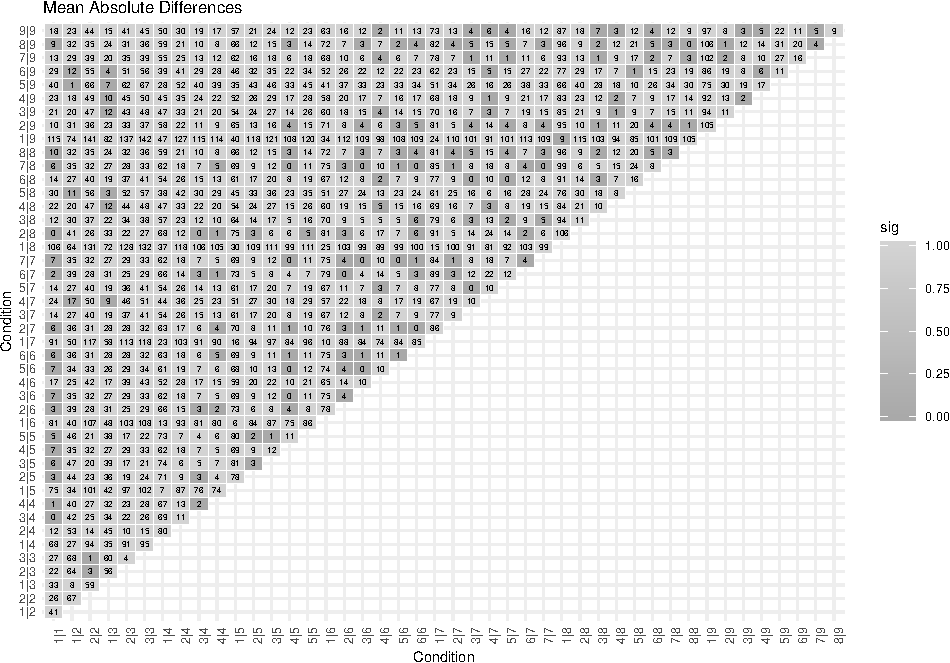
\includegraphics{Entropy_typing_draft_files/figure-latex/typing_mean_iksis_comparisons-1.pdf}
\caption{}
\end{figure}

Our more important aim was to determine whether variation among these
means can be explained by variation in letter uncertainty. For this
reason we do not exhaustively discuss all of the possible 990
differences among these 45 conditions. Nevertheless, we did conduct all
990 comparisons using bonferroni corrected paired samples t-tests. The
results are displayed Figure 2, which shows absolute mean differences
between conditions color coded for significance (light grey is
significant).

\subsection{Letter Uncertainty by position and word
length}\label{letter-uncertainty-by-position-and-word-length}

The primary question of interest was whether natural variation in letter
uncertainty explains variance in mean IKSI by position and word length.
We estimated letter uncertainty by position and word length from
google's ngram database, which provides frequency counts of letters and
words occuring in Google's massive corpus (X million) of digitized
books. Letter frequency counts for letters a to z, for each position in
words from length one to nine, were obtained from Norvig ().

For each letter frequency distribution, we computed Shannon's H
(entropy) to quantify letter uncertainty.

We converted each letter frequency distribution to a probability
distribution then calculated H for each distribution. Figure 3 displays
estimates of letter uncertainty (H) as a function of letter position and
word length. Visual inspection of the graph shows that variation in
letter uncertainty maps closely onto variation in mean IKSI (Figure 1)
as a function of position and word length. In particular, letter
uncertainty and mean IKSI for position one as a function of word length
appear highly similar. And for the remaining positions, letter
uncertainty shows an inverted U- shape with greater letter uncertainty
in the middle rather than the beginning and endings of words. This
suggests that natural variation of letter uncertainty across position
and word in English may account for aspects of the first-letter and
mid-word slowing phenomena in typing.

\subsection{Letter Uncertainty and Mean
IKSI}\label{letter-uncertainty-and-mean-iksi}

If the Hick-Hyman law applied to continuous typing we would expect a
neat linear relationship between mean IKSIs and letter uncertainty.
Figure 4 shows a plot of mean IKSIs taken from all positions and word
lengths against letter uncertainty. The scatterplot shows a general
trend for mean IKSI to increase as a function of letter uncertainty.

\begin{figure}[htbp]
\centering
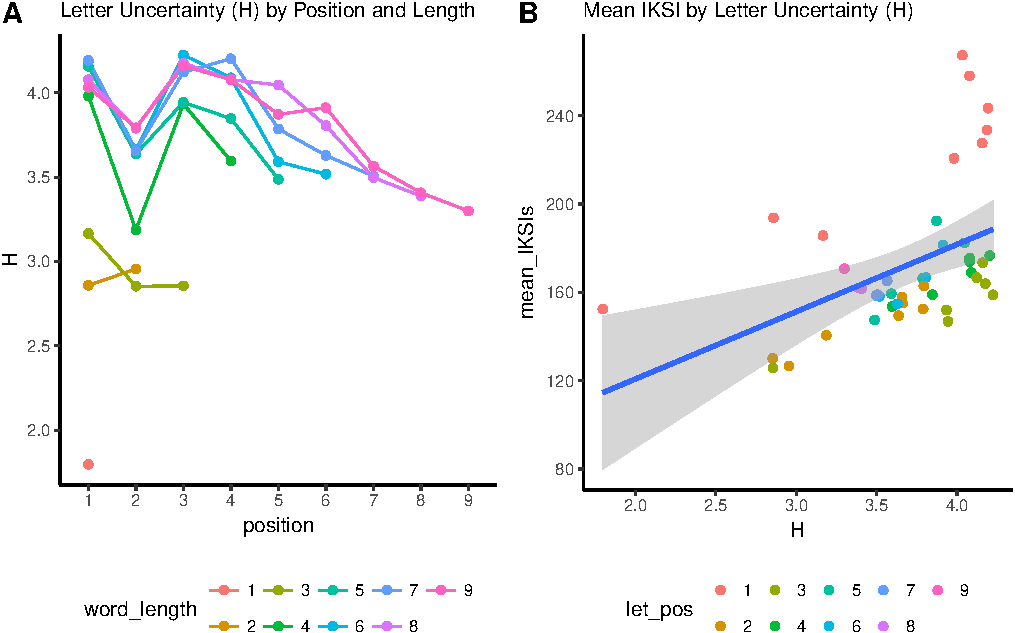
\includegraphics{Entropy_typing_draft_files/figure-latex/letter_uncertainty_by_IKSI-1.pdf}
\caption{}
\end{figure}

A linear regression with group mean IKSIs (collapsed over subjects) as
the dependent variable, and letter uncertainty as the independent
variable showed a significant positive trend, F(1, 43) = 11.82, p =
0.0013, \(R^2 =\) 0.22 ( meanIKSI = 59.75 \(+\) 30.49 \(* H\) ). We also
conducted separate linear regressions for each subject and found similar
results. For example, the mean correlation was r = 0.44 (SE = 0.0085);
mean \(R^2\) = 0.22 (SE = 0.0072); and mean p = 0.047 (SE = 0.0072).

\subsection{Interim Discussion}\label{interim-discussion}

We can conclude that letter uncertainty as a function of position and
length explains a small amount variation in mean IKSIs during continuous
typing. The present analysis does not provide strong evidence that a
process sensitive to letter uncertainty causes both first-letter and
mid-word slowing. For example, all of the first position mean IKSIs are
longer than mean IKSIs for other positions at comparables levels of
letter uncertainty. And, a linear regression on the group mean IKSIs
including letter uncertainty and position (first letter vs.~other
letter) as independent variables explains much more variance, \(R^2\) =
0.86, p \textless{} .001, than the regression only including letter
uncertainty.

This pattern invites a dual-process interpretation. For example,
first-letter slowing could be explained by a planning process that
increases first position IKSIs as a function of word length. Longer
words have more letters, thus plan construction and buffering is assumed
to take more time before sequence production begins. At the same time,
the finding that letter uncertainty does explain some variance in mean
IKSI across position suggests that sequence production is also
influenced by a process sensitive to letter uncertainty.

\subsection{Letter Uncertainty by position, word length, and n-1 letter
identity}\label{letter-uncertainty-by-position-word-length-and-n-1-letter-identity}

Determining whether first-letter and mid-word slowing could emerge from
a process sensitive to letter uncertainty depends on how letter
uncertainty is calculated. Letter uncertainty can be calculated from any
discrete probability distribution of letters. In the previous section we
somewhat arbitrarily calculated letter uncertainty separately for each
letter position in words of length one to nine. However, the number of
alternative schemes is vast. For example, we could further
conditionalize our postion by word length probability distributions by
the letter identities of letters occuring in any position n-1 to n-x, or
n+1 to n+y of a specific position. Furthermore, we could conditionalize
letter distributions upon any permissible number of preceding or
succeeding n-grams (groups of letters).

Although an exhaustive calculation of letter uncertainty is beyond the
scope of this paper, we nevertheless took one further step and
calculated letter uncertainty by position and word length,
conditionalizing upon n-1 letter identity. Fortunately, Norvig () also
provided bigram frequency counts from the google ngram corpus as a
function of position and word length. We calculated letter uncertainty
in the following manner. First position letters have no preceding
letter, so H as a function of word length was identical to our prior
calculation. For letters in positions two to nine, for all word lengths,
we calculated H for every n-1 letter identity, and then took the mean H
for each position and length. For example, the second position of a
two-letter word has a maximum of 26 letter probability distributions,
one for each possible n-1 letter (a to z). We calculated H for all n-1
distributions, then took the mean H as our measure of letter uncertainty
for each position and word length. Figure X shows mean H conditionalized
by n-1 letter identity, as a function of letter position and word
length.

\begin{figure}[htbp]
\centering
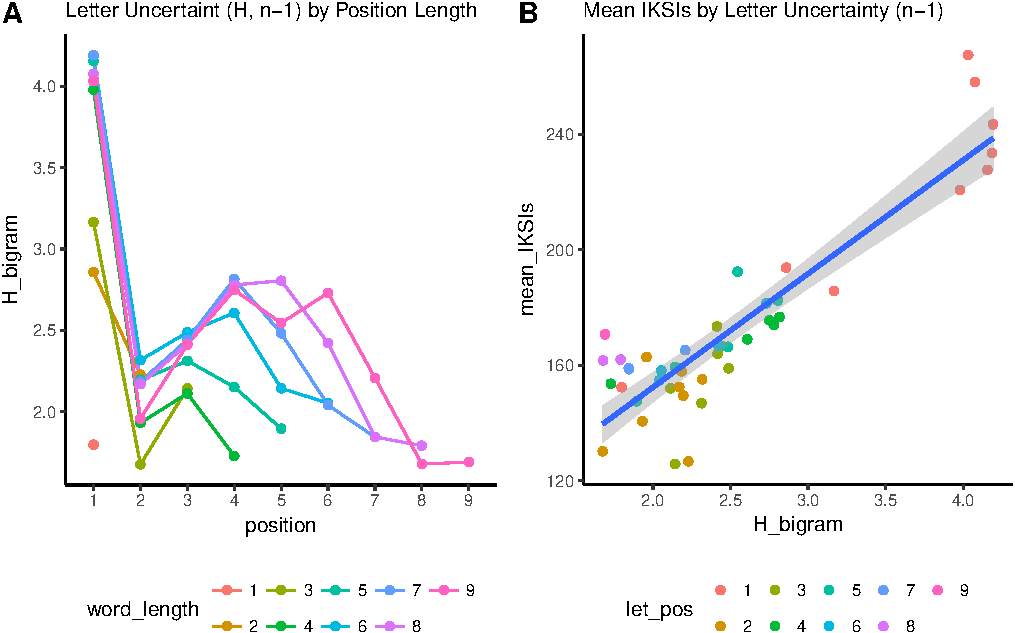
\includegraphics{Entropy_typing_draft_files/figure-latex/letter_uncertainty_bigram-1.pdf}
\caption{}
\end{figure}

Unsurprisingly, letter identity becomes more predictable when n-1 letter
identity is known. Compared to the letter uncertainty measures in Figure
X, we see that H for letters in positions two to nine is much lower when
n-1 letter identity is taken into account. More important, the pattern
of H in Figure X much more closely resembles the pattern of mean IKSIs
in Figure X.

Figure X displays a scatterplot of mean IKSIs as a function of letter
uncertainty conditionalized by letter n-1 identity across positions and
word length. A linear regression on mean IKSIs using our new measure of
letter uncertainty as the independent variable showed a strong positive
relationship, F(1, 43) = 182.44, p = 4.5e-17, \(R^2 =\) 0.81 ( meanIKSI
= 73.72 \(+\) 39.31 \(* H\) ).

\section{Discussion}\label{discussion}

\section{An instance-based model}\label{an-instance-based-model}

We have shown that variation in mean IKSIs as a function of letter
position and word length can be well explained by natural variation in
letter uncertainty conditionalized by letter n-1 identity by letter
position and word length. This finding licenses consideration of the
claim that first-letter and mid-word slowing are caused by a single
process sensitive to letter uncertainty. However, the plausibility of
this causal claim is empty in the absence of a working process model.
Next, we establish theoretical plausibility by showing that letter
uncertainty influences on performance can be explained in terms of
Logan's (1988) instance-based memory model of automatization.

Instance theory provides an account of how performance becomes
automatized with practice. Among other things, it provides a theoretical
explanation of learning curves that follow a power function (). We will
show that the instance theory process also develops sensitivity to
uncertainty in the stimuli it encounters over practice. More
specifically, instance theories predictions for performance are nearly
identical to the hick-hyman law which posits that reaction times are a
linear function of the uncertainty in a choice set.

Instance theory models learning as a function of practice in terms of
cue-driven retrieval of stored memory traces. A new unique trace is
preserved in memory every time a response is given to a stimulus. When a
familiar stimulus is encountered again, it automatically triggers the
retrieval of all stored instances of the stimulus. The timing of the
memory-based response to a current stimulus is treated as a race.
Whichever memory trace is retrieved first wins the race. As a result,
the memory-based reaction time to respond to a stimulus is determined by
the retrieval time associated with the fastest memory trace for that
stimulus. The retrieval times for every memory trace are assumed to
vary, and can be sampled from any desired distribution.

So, instance theory models practice based performance speed-ups in terms
of sampling extreme values from a growing retrieval time distribution.
As the number of memory traces grows the range of the retrieval time
distribution also grows. As a result, the minimum value of the
distribution (fastest retrieval) is more likely to be smaller for
distributions with more than fewer memory traces. In other words,
reaction times will tend to be faster for higher than lower frequency
stimuli.

We can now draw a more transparent connection between instance theory
and information theory. Information theory provides H as a summary
statistic of probability distributions for any discrete set of stimuli.
Empirical probability distributions for natural occuring stimuli, such
as letters, are found by counting stimulus frequencies, and then
dividing a stimulus frequency distribution by it's sum. Instance
theories predictions for response times in a stimulus set will be
monotonically decreasing as a function of each stimulus frequencies. We
should also expect that a summary statistic of instance theories
predictions for mean reaction time, collapsing across all items in the
set, will behave in a similar manner to information theory's summary
statistic, which also collapses over the expected frequency of each item
in the set. We demonstrate these relationships by monte-carlo
simulation.

Our goal was to model instance theory predictions for keystroke
production times for typing natural english sentences as a function of
letter position and word length. We treated all 26 letters that could
possibly occur in any position for any word length as completely unique
and independent stimuli. We modeled the structure of natural english
using the 45 letter probability distributions derived from Norvig's
letter frequence counts by position and word length, from Google's
n-gram corpus.

We modelled keystroke times for specific letters in the following
manner. At different practice intervals each letter, occuring in each
position for each word length, had occured in the model's history with
specific frequency. We estimated reaction time as a function of
frequency by monte-carlo simulation. We assumed that the retrieval time
distribution for each stimulus was sampled from a normal distribution
with mean = 500, and standard deviation = 100. Using R, we sampled
retrieval times from the normal distribution n times, where n was the
current number of memory traces. Then we took the minimum value from the
sampling distribution as the reaction time. We repeated this process
1000 times to estimate the expected mean reaction time (expected minimum
retrieval time) for the given frequency value. In this way, we estimated
mean keystroke production times for every letter position across
different word lengths. Last, we evaluated model predictions across four
practice intervals.

Figure X displays the instance model predictions, across increasing
amounts of practice, for mean keystroke production times as a function
of letter position and word length. As expected, simulated keystroke
times shorten with practice. More imporant, at each stage in practice,
simulated keystroke times show the same qualitative pattern of variation
across letter postion and word length. Notably, these appear very
similar to human typing performance, and to letter uncertainty as a
function of position and word length.

Finally, we conducted linear regressions on simulated mean typing times
using letter uncertainty as the independent variable. We found that
letter uncertainty nearly perfectly explains the variance in simulated
keystroke time, with R\^{}2 increasing across practice.

\section{Conclusion}\label{conclusion}

Future studies should investigate the role of probability of repetition
in regulating response times.\\
Kornblum in 1969 found that with constant H, trials that had higher
chances of sequentially repeating stimuli experienced faster response
times.

\newpage

\section{References}\label{references}

\begingroup
\setlength{\parindent}{-0.5in} \setlength{\leftskip}{0.5in}

\hypertarget{refs}{}
\hypertarget{ref-R-papaja}{}
Aust, F., \& Barth, M. (2018). \emph{papaja: Create APA manuscripts with
R Markdown}. Retrieved from \url{https://github.com/crsh/papaja}

\hypertarget{ref-R-magrittr}{}
Bache, S. M., \& Wickham, H. (2014). \emph{Magrittr: A forward-pipe
operator for r}. Retrieved from
\url{https://CRAN.R-project.org/package=magrittr}

\hypertarget{ref-clark_supersizing_2008}{}
Clark, A. (2008). \emph{Supersizing the mind: Embodiment, action, and
cognitive extension}. OUP USA. Retrieved from
\url{https://books.google.com/books?hl=en\&lr=\&id=n5wRDAAAQBAJ\&oi=fnd\&pg=PR9\&dq=andy+clark\&ots=_Cpl448Qox\&sig=SC8xkxJaEf7G8EZaGPS0zSDEQX8}

\hypertarget{ref-R-Crump}{}
Crump, M. (2017). \emph{Crump: Crump lab functions}.

\hypertarget{ref-R-data.table}{}
Dowle, M., \& Srinivasan, A. (2017). \emph{Data.table: Extension of
`data.frame`}. Retrieved from
\url{https://CRAN.R-project.org/package=data.table}

\hypertarget{ref-R-RcppZiggurat}{}
Eddelbuettel, D. (2017). \emph{RcppZiggurat: 'Rcpp' integration of
different ``ziggurat'' normal rng implementations}. Retrieved from
\url{https://CRAN.R-project.org/package=RcppZiggurat}

\hypertarget{ref-R-Rcpp_b}{}
Eddelbuettel, D., \& Balamuta, J. J. (2017). Extending extitR with
extitC++: A Brief Introduction to extitRcpp. \emph{PeerJ Preprints},
\emph{5}, e3188v1.
doi:\href{https://doi.org/10.7287/peerj.preprints.3188v1}{10.7287/peerj.preprints.3188v1}

\hypertarget{ref-R-Rcpp_a}{}
Eddelbuettel, D., \& François, R. (2011). Rcpp: Seamless R and C++
integration. \emph{Journal of Statistical Software}, \emph{40}(8),
1--18.
doi:\href{https://doi.org/10.18637/jss.v040.i08}{10.18637/jss.v040.i08}

\hypertarget{ref-fodor_modularity_1983}{}
Fodor, J. A. (1983). \emph{The modularity of mind: An essay on faculty
psychology}. Cambridge, Mass.: MIT Press.

\hypertarget{ref-heath_stochastic_1990}{}
Heath, R. A., \& Willcox, C. H. (1990). A stochastic model for
inter-keypress times in a typing task. \emph{Acta Psychologica},
\emph{75}(1), 13--39.

\hypertarget{ref-JacobyNonanalyticcognitionMemory1984}{}
Jacoby, L. L., \& Brooks, L. R. (1984). Nonanalytic cognition: Memory,
perception, and concept learning. \emph{The Psychology of Learning and
Motivation}, \emph{18}, 1--47.

\hypertarget{ref-john_typist:_1996}{}
John, B. E. (1996). TYPIST: A theory of performance in skilled typing.
\emph{Human-Computer Interaction}, \emph{11}(4), 321--355.

\hypertarget{ref-R-ggpubr}{}
Kassambara, A. (2017). \emph{Ggpubr: 'Ggplot2' based publication ready
plots}. Retrieved from \url{https://CRAN.R-project.org/package=ggpubr}

\hypertarget{ref-KolersProceduresmind1984}{}
Kolers, P. A., \& Roediger, H. L. (1984). Procedures of mind.
\emph{Journal of Verbal Learning and Verbal Behavior}, \emph{23}(4),
425--449.

\hypertarget{ref-logan_toward_1988}{}
Logan, G. D. (1988). Toward an instance theory of automatization.
\emph{Psychological Review}, \emph{95}(4), 492--527. Retrieved from
\url{http://psycnet.apa.org/journals/rev/95/4/492/}

\hypertarget{ref-logan_hierarchical_2011}{}
Logan, G. D., \& Crump, M. J. C. (2011). Hierarchical control of
cognitive processes: The case for skilled typewriting. In B. H. Ross
(Ed.), \emph{Psychology of Learning and Motivation} (Vol. 54, pp.
1--27). Elsevier. Retrieved from
\href{https://CrumpLab.github.io/CognitionPerformanceLab/CrumpPubs/Logan\%20and\%20Crump\%20-\%202011.pdf}{https://CrumpLab.github.io/CognitionPerformanceLab/CrumpPubs/Logan and Crump - 2011.pdf}

\hypertarget{ref-R-skimr}{}
McNamara, A., Arino de la Rubia, E., Zhu, H., Ellis, S., \& Quinn, M.
(2018). \emph{Skimr: Compact and flexible summaries of data}. Retrieved
from \url{https://CRAN.R-project.org/package=skimr}

\hypertarget{ref-R-bindrcpp}{}
Müller, K. (2018). \emph{Bindrcpp: An 'rcpp' interface to active
bindings}. Retrieved from
\url{https://CRAN.R-project.org/package=bindrcpp}

\hypertarget{ref-R-bit64}{}
Oehlschlägel, J. (2017). \emph{Bit64: A s3 class for vectors of 64bit
integers}. Retrieved from \url{https://CRAN.R-project.org/package=bit64}

\hypertarget{ref-R-bit}{}
Oehlschlägel, J. (2018). \emph{Bit: A class for vectors of 1-bit
booleans}. Retrieved from \url{https://CRAN.R-project.org/package=bit}

\hypertarget{ref-OstryDeterminantsinterkeytimes1983}{}
Ostry, D. J. (1983). Determinants of interkey times in typing.
\emph{Cognitive Aspects of Skilled Typewriting}, 225--246.

\hypertarget{ref-R-Rfast}{}
Papadakis, M., Tsagris, M., Dimitriadis, M., Fafalios, S., Tsamardinos,
I., Fasiolo, M., \ldots{} Lakiotaki, K. (2018). \emph{Rfast: A
collection of efficient and extremely fast r functions}. Retrieved from
\url{https://CRAN.R-project.org/package=Rfast}

\hypertarget{ref-R-base}{}
R Core Team. (2017). \emph{R: A language and environment for statistical
computing}. Vienna, Austria: R Foundation for Statistical Computing.
Retrieved from \url{https://www.R-project.org/}

\hypertarget{ref-R-rlist}{}
Ren, K. (2016). \emph{Rlist: A toolbox for non-tabular data
manipulation}. Retrieved from
\url{https://CRAN.R-project.org/package=rlist}

\hypertarget{ref-rumelhart_parallel_1986}{}
Rumelhart, D. E., \& McClelland, J. L. (1986). \emph{Parallel
distributed processing, Explorations in the microstructure of cognition,
Volume 1: Foundations}. Cambridge, Mass. {[}u.a.{]}: MIT Press.

\hypertarget{ref-RumelhartSimulatingskilledtypist1982}{}
Rumelhart, D. E., \& Norman, D. A. (1982). Simulating a skilled typist:
A study of skilled cognitive-motor performance. \emph{Cognitive
Science}, \emph{6}(1), 1--36.

\hypertarget{ref-salthouse_perceptual_1986}{}
Salthouse, T. A. (1986). Perceptual, cognitive, and motoric aspects of
transcription typing. \emph{Psychological Bulletin}, \emph{99}(3),
303--319.

\hypertarget{ref-Shannonmathematicaltheorycommunication1998}{}
Shannon, C. E., \& Weaver, W. (1998). \emph{The mathematical theory of
communication}. University of Illinois press.

\hypertarget{ref-R-ggplot2}{}
Wickham, H. (2009). \emph{Ggplot2: Elegant graphics for data analysis}.
Springer-Verlag New York. Retrieved from \url{http://ggplot2.org}

\hypertarget{ref-R-dplyr}{}
Wickham, H., Francois, R., Henry, L., \& Müller, K. (2017). \emph{Dplyr:
A grammar of data manipulation}. Retrieved from
\url{https://CRAN.R-project.org/package=dplyr}

\hypertarget{ref-will_linguistic_2006}{}
Will, U., Nottbusch, G., \& Weingarten, R. (2006). Linguistic units in
word typing: Effects of word presentation modes and typing delay.
\emph{Written Language \& Literacy}, \emph{9}(1), 153--176.

\hypertarget{ref-wu_queuing_2008}{}
Wu, C., \& Liu, Y. (2008). Queuing Network Modeling of Transcription
Typing. \emph{ACM Transactions on Computer-Human Interaction},
\emph{15}(1), 1--45.
doi:\href{https://doi.org/10.1145/1352782.1352788}{10.1145/1352782.1352788}

\hypertarget{ref-R-knitr}{}
Xie, Y. (2015). \emph{Dynamic documents with R and knitr} (2nd ed.).
Boca Raton, Florida: Chapman; Hall/CRC. Retrieved from
\url{https://yihui.name/knitr/}

\endgroup






\end{document}
